\documentclass[UTF8,11pt]{ctexart}

\usepackage[margin=1in]{geometry}
\usepackage{amsmath, amssymb}
\usepackage{booktabs}
\usepackage{float}
\usepackage{graphicx}
\usepackage{hyperref}

\title{使用 SAT/SMT 编码求解整数方形与矩形装箱问题}
\author{CS 517 Final Project Team}
\date{\today}

\begin{document}

\maketitle

\begin{abstract}
本文研究一个基于整数网格的二维装箱问题：给定一个矩形容器，以及一组边长为整数的方形或矩形，判断是否能够将所有物体放入容器并且互不重叠。二维装箱问题是经典的 NP-hard 组合优化问题，在制造业、切割下料、物流装载、存储分配、自动化设计以及 VLSI 芯片布局等领域都有实际意义。本项目的重点不是重新证明 NP-hardness，而是实现从装箱实例到 SAT/SMT 公式的规约：每个可满足赋值对应一个合法装箱方案，反之每个合法装箱方案也对应一个可满足赋值。我们使用 Z3 实现 SMT 求解器，从整数方形装箱 baseline 扩展到支持可选 90 度旋转的矩形装箱，并生成实验数据和可视化结果。
\end{abstract}

\section{引言}

装箱问题要求把一组物体放入有限空间中，同时保证物体之间不发生重叠。即使在二维、整数、轴对齐等限制条件下，许多相关问题仍然具有较高的计算复杂度。二维矩形装箱、bin packing 和 cutting stock 等问题已经在近似算法和组合优化中被广泛研究 \cite{garey1979computers,coffman1980performance}。

我们的项目从整数方形装箱开始，先实现一个简单但完整的 baseline，然后把同一套建模思想扩展到矩形装箱，并进一步允许矩形旋转 90 度。老师在 proposal 后反馈说，扩展到 squares 之外会更有趣；因此我们选择矩形加旋转作为最终扩展方向。这个方向仍然和原始问题共享同一类 SMT 约束，同时可以展示旋转变量如何改变可满足性和求解难度。

\section{问题定义}

基础版本的整数方形装箱问题输入为：
\begin{itemize}
    \item 一个边长为 \(L \in \mathbb{N}\) 的正方形容器；
    \item 一组方形边长 \(s_1,s_2,\ldots,s_n\)，其中每个 \(s_i \in \mathbb{N}\)。
\end{itemize}

每个方形必须轴对齐放置，其左下角坐标为整数 \((x_i,y_i)\)。合法解需要满足两个条件：
\begin{enumerate}
    \item 每个方形完全位于 \(L\times L\) 容器内部；
    \item 任意两个方形不重叠。
\end{enumerate}

本项目实现的工具支持三种模式：
\begin{itemize}
    \item \texttt{squares}：所有物体都是方形，容器也是方形；
    \item \texttt{rectangles\_no\_rotation}：物体是矩形，但方向固定；
    \item \texttt{rectangles\_rotation}：物体是矩形，并且每个矩形可以选择是否旋转 90 度。
\end{itemize}

本文主要求解决策问题：是否存在一个合法装箱方案。如果 Z3 返回 SAT，我们还会从模型中读出每个物体的位置和旋转状态，并绘制装箱图。

\section{SAT 编码思路}

一种直接的 SAT 规约方式是枚举所有合法位置，并为每个物体的每个位置创建一个布尔变量。对于方形 \(i\)，它的合法位置集合为：
\[
P_i = \{(a,b) \mid 0 \leq a \leq L-s_i,\ 0 \leq b \leq L-s_i\}.
\]

对每个 \(p\in P_i\)，引入布尔变量 \(X_{i,p}\)，表示方形 \(i\) 是否放在位置 \(p\)。然后添加两类约束：
\begin{itemize}
    \item exactly-one 约束：每个方形必须且只能选择一个位置；
    \item non-overlap 约束：如果两个位置对应的方形会重叠，则它们不能同时被选择。
\end{itemize}

具体来说，每个方形至少选择一个位置：
\[
\bigvee_{p\in P_i} X_{i,p}.
\]
每个方形至多选择一个位置：
\[
\neg X_{i,p} \vee \neg X_{i,q}
\]
其中 \(p\neq q\)。如果方形 \(i\) 在位置 \(p\) 和方形 \(j\) 在位置 \(q\) 会重叠，则加入：
\[
\neg X_{i,p} \vee \neg X_{j,q}.
\]

这个 SAT 公式可满足当且仅当原始装箱实例有合法解。SAT 编码的优点是逻辑结构直观，缺点是需要枚举所有位置，变量数量可能很大。因此实际实现中我们使用更紧凑的 SMT 编码。

\section{SMT 编码}

我们的实现使用 Z3 的整数算术接口 \cite{deMoura2008z3}。对每个物体 \(i\)，创建两个整数变量：
\[
x_i,\ y_i.
\]
它们表示物体左下角的位置。

\subsection{矩形尺寸与旋转变量}

对于不可旋转的矩形 \(i\)，有效宽高就是输入宽高：
\[
W_i=w_i,\qquad H_i=h_i.
\]

对于可旋转矩形，引入一个布尔变量 \(r_i\)。如果 \(r_i\) 为 false，则矩形保持原方向；如果 \(r_i\) 为 true，则矩形旋转 90 度：
\[
W_i =
\begin{cases}
w_i & \text{if } \neg r_i,\\
h_i & \text{if } r_i,
\end{cases}
\qquad
H_i =
\begin{cases}
h_i & \text{if } \neg r_i,\\
w_i & \text{if } r_i.
\end{cases}
\]

在 Z3 中，\(W_i\) 和 \(H_i\) 使用条件表达式表示。方形不需要旋转变量，因为旋转不会改变它的形状。

\subsection{边界约束}

对每个物体 \(i\)，我们添加：
\[
0 \leq x_i,\quad 0 \leq y_i,
\]
\[
x_i+W_i \leq C_W,\quad y_i+H_i \leq C_H.
\]
其中 \(C_W\) 和 \(C_H\) 是容器的宽和高。这些约束保证每个物体完全位于容器内部。

\subsection{不重叠约束}

对任意两个不同物体 \(i,j\)，它们必须满足四种相对位置之一：\(i\) 在 \(j\) 左侧，\(j\) 在 \(i\) 左侧，\(i\) 在 \(j\) 下方，或 \(j\) 在 \(i\) 下方。因此加入：
\[
(x_i+W_i \leq x_j)
\vee
(x_j+W_j \leq x_i)
\vee
(y_i+H_i \leq y_j)
\vee
(y_j+H_j \leq y_i).
\]

该 SMT 公式使用 \(2n\) 个整数坐标变量，最多 \(n\) 个布尔旋转变量，\(4n\) 个边界不等式，以及 \(\binom{n}{2}\) 个 pairwise non-overlap 约束。

\subsection{正确性}

如果 SMT 公式可满足，那么模型会给出每个物体的坐标和旋转状态。边界约束保证物体不越界，不重叠约束保证任意两个矩形水平或垂直分离，因此模型对应一个合法装箱方案。

反过来，如果原始装箱实例存在合法方案，那么可以把每个物体的坐标赋给 \(x_i,y_i\)，并根据是否旋转赋给 \(r_i\)。这个赋值会满足所有边界约束和不重叠约束。因此 SMT 公式可满足当且仅当装箱实例有解。

\section{优化与实现细节}

实现中加入了几个简单但有效的处理：
\begin{itemize}
    \item 面积下界：如果所有物体总面积超过容器面积，则直接返回 UNSAT；
    \item 按面积降序建模：先处理大物体，方便 solver 更早面对关键约束；
    \item 可选对称性破缺：把最大物体限制在左下半区域，以减少通过水平或垂直翻转得到的等价搜索空间；
    \item JSON 输入：支持容器尺寸、物体尺寸、是否可旋转、timeout 和 symmetry breaking 设置；
    \item 可视化：对 SAT 结果输出 PNG，对 UNSAT/UNKNOWN 结果也生成对应图像。
\end{itemize}

项目代码主要分为四个模块：\texttt{packing\_solver.py} 负责 Z3 编码和结果验证，\texttt{instances.py} 负责 JSON 和随机实例，\texttt{visualize.py} 负责绘图，\texttt{experiments.py} 负责批量实验和 CSV 输出。

\section{实验}

实验入口为：
\[
\texttt{python -m src.experiments --preset final}.
\]
该命令会生成 \texttt{results/summary.csv}、单个实例图片，以及两张论文用汇总图。

\subsection{方形 baseline}

方形 baseline 使用固定的方形列表：
\[
[5,4,3,3,3,2,2,2,2,1,1,1,1].
\]
我们改变容器边长 \(L\)，观察 SAT/UNSAT 结果和运行时间。

\begin{table}[H]
\centering
\begin{tabular}{rrrrlr}
\toprule
\(L\) & 物体数 & 总面积 & 容器面积 & 结果 & 时间(s) \\
\midrule
30 & 13 & 88 & 900 & SAT & 0.0097 \\
25 & 13 & 88 & 625 & SAT & 0.0079 \\
20 & 13 & 88 & 400 & SAT & 0.0088 \\
15 & 13 & 88 & 225 & SAT & 0.0131 \\
12 & 13 & 88 & 144 & SAT & 0.0107 \\
11 & 13 & 88 & 121 & SAT & 0.0094 \\
10 & 13 & 88 & 100 & SAT & 0.0275 \\
9  & 13 & 88 & 81  & UNSAT & 0.0000 \\
\bottomrule
\end{tabular}
\caption{方形 baseline 实验结果。\(L=9\) 时总面积 88 大于容器面积 81，因此由面积下界直接判定为 UNSAT。}
\end{table}

\begin{figure}[H]
\centering
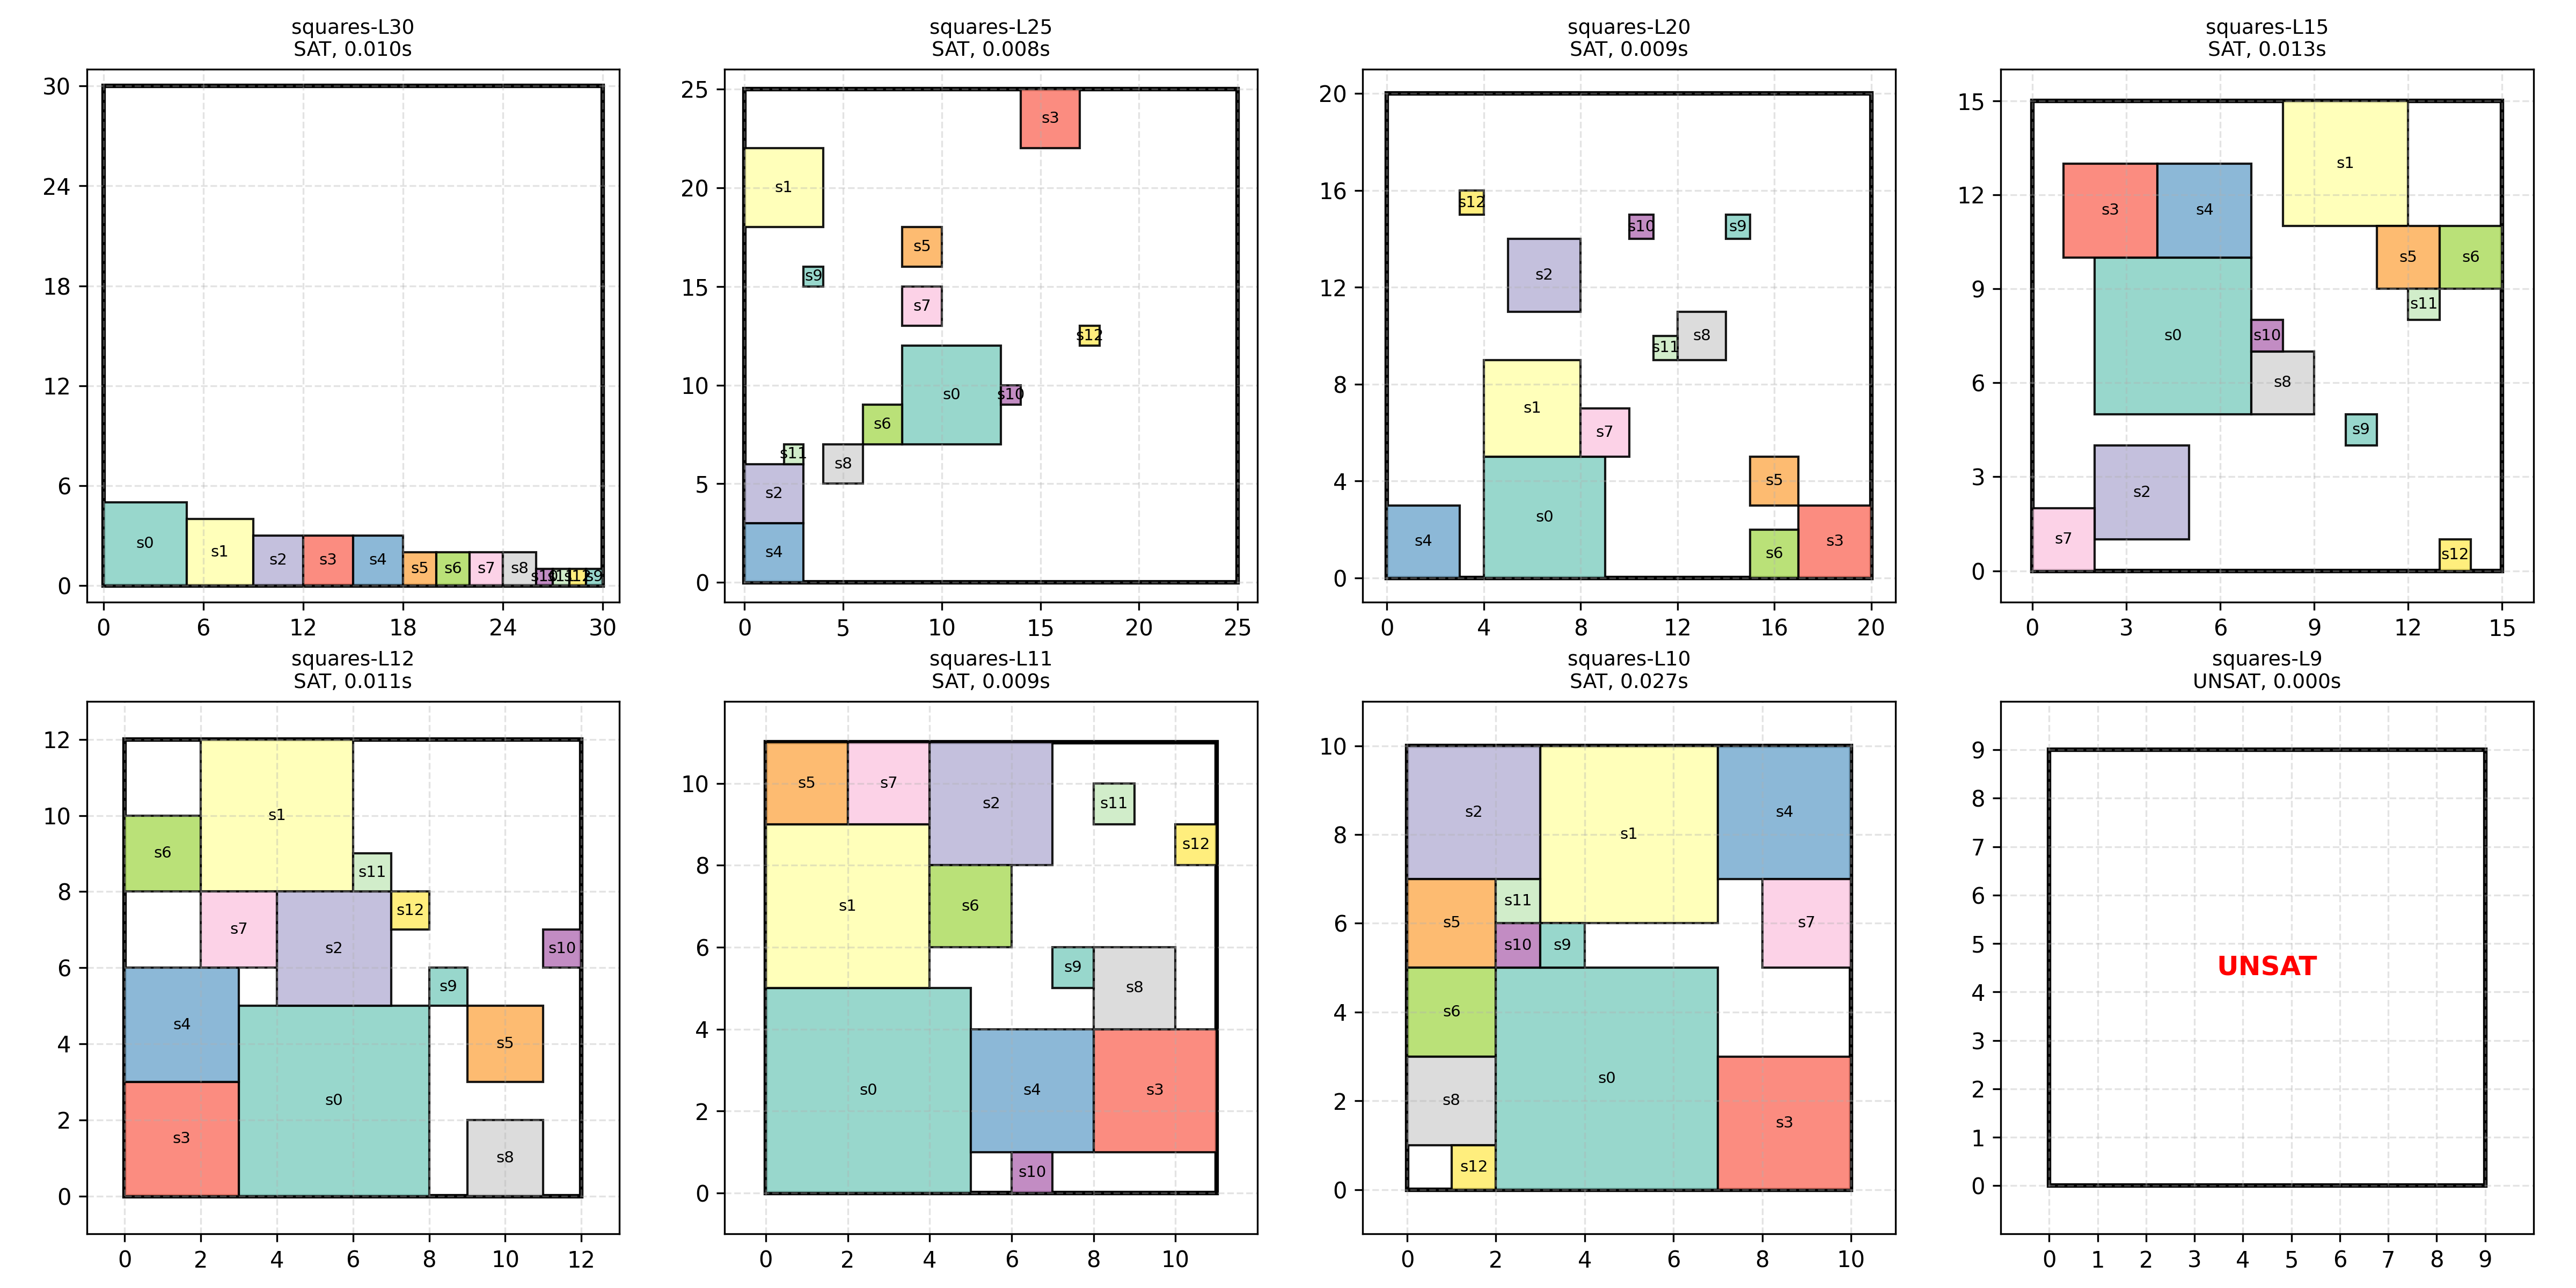
\includegraphics[width=0.95\textwidth]{../results/square_baseline_grid.png}
\caption{方形 baseline 的可视化结果。}
\end{figure}

\subsection{矩形与旋转实验}

矩形实验使用同一组物体，在不允许旋转和允许旋转两种模式下比较结果。这个实验直接展示了旋转变量的作用：它可能改变问题的可满足性，但也会增加 solver 的搜索空间。

\begin{table}[H]
\centering
\begin{tabular}{rrllrr}
\toprule
物体数 & 密度 & 不旋转 & 可旋转 & 不旋转时间 & 可旋转时间 \\
\midrule
4 & 0.6333 & SAT & SAT & 0.0026 & 0.0028 \\
5 & 0.7667 & SAT & SAT & 0.0034 & 0.0048 \\
6 & 0.8500 & SAT & SAT & 0.0050 & 0.0074 \\
7 & 0.9250 & SAT & SAT & 0.0067 & 0.0079 \\
8 & 0.9917 & UNSAT & SAT & 0.0068 & 0.2816 \\
\bottomrule
\end{tabular}
\caption{矩形实验结果。最关键的是 \(n=8\) 的实例：不允许旋转时 UNSAT，允许旋转时 SAT。}
\end{table}

\begin{figure}[H]
\centering
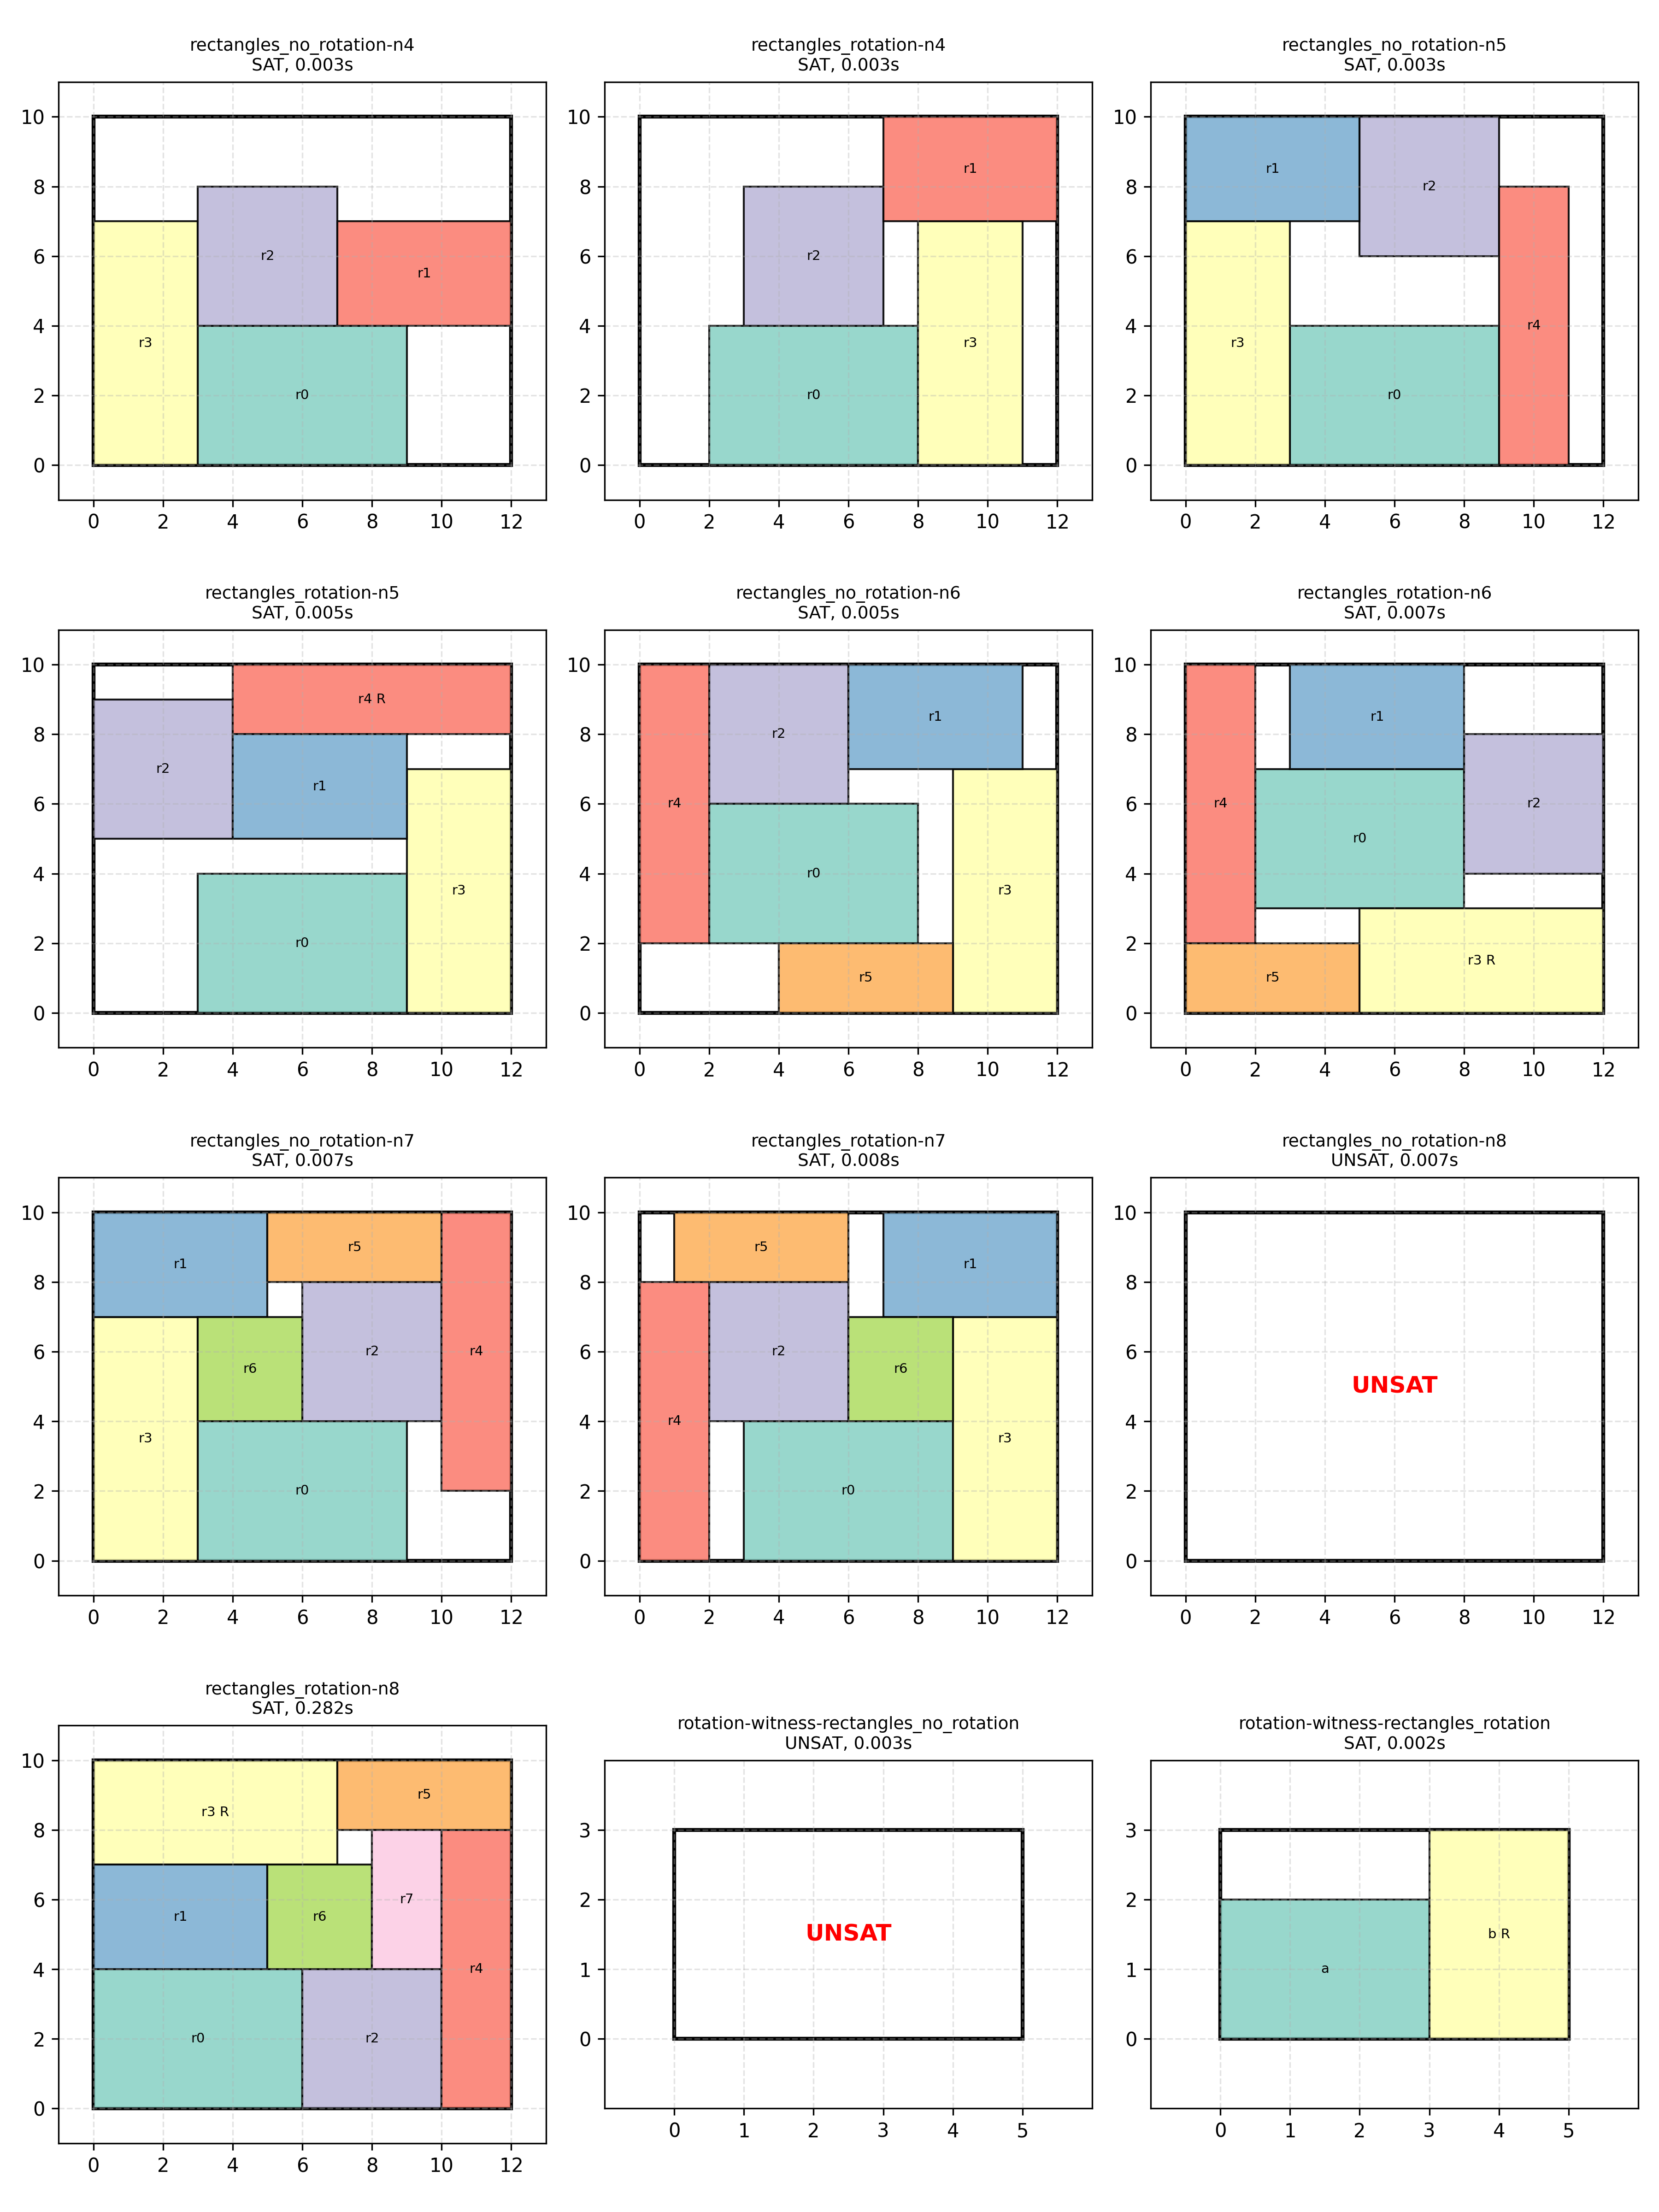
\includegraphics[width=0.95\textwidth]{../results/rectangle_experiments_grid.png}
\caption{矩形实验可视化：比较固定方向和可选旋转。}
\end{figure}

\subsection{密度扩展实验}

随机实验使用固定 seed 生成矩形实例，并逐渐增加物体数量。主要输入维度包括物体数 \(n\)、容器尺寸 \(C_W,C_H\)、物体尺寸分布、密度 \(\sum_i w_i h_i/(C_WC_H)\)，以及是否允许旋转。实验中，密度超过 1 的实例会被面积下界直接判定为 UNSAT；接近可行边界的实例通常更有分析价值，因为 solver 需要在有限空间中搜索更多冲突关系。

\section{团队分工}

Changqing Li 负责 SMT 规约部分，包括坐标变量、旋转变量、不重叠约束和正确性论证。Fei Keng 负责 Python 工具实现，包括 JSON 解析、测试实例生成、实验 runner 和可视化。Grant O'Connor 负责背景研究和实验结果写作，包括装箱问题在制造、物流、芯片设计等领域的意义，以及论文整理。

\section{结论}

本项目展示了如何把二维装箱问题规约为 SAT/SMT 公式，并使用 Z3 求解。方形装箱可以通过枚举位置得到 SAT 编码，也可以通过整数坐标变量得到更紧凑的 SMT 编码。我们进一步把 SMT 编码扩展到矩形，并通过布尔旋转变量支持 90 度旋转。实验结果显示，旋转不仅是一个自然的建模扩展，而且确实可能改变实例的 SAT/UNSAT 结果。最终工具支持 JSON 输入、可复现实验、CSV 输出和图像可视化，能够满足课程项目对 problem-to-SMT reduction、实验分析和结果展示的要求。

\bibliographystyle{plain}
\bibliography{references}

\end{document}

